% 原文PDF167--187頁（本文145--165頁）、第5章全文・演習。
\sectionlink{弦のS行列}\label{ch:5}

第3章では、弦の $S$ 行列を、頂点演算子を伴うコンパクトな二次元曲面についての経路積分として書いた。この章では、その経路積分をゲージ固定した形に帰着させる。

\subsectionlink{円とトーラス}\label{sec:5.1}

図3.7のように、$(\mathrm{diff}\times\mathrm{Weyl})$ 等価な各集合から一つの配置を選ぶ、ゲージ切片を定めたい。局所的には計量を固定することでこれを行ったが、大域的には、計量の空間と世界面のゲージ群の間に小さな不一致がある。

ここでも、点粒子がよい例を与える。Euclid 経路積分
\begin{equation}
\int[de\,dX]\exp\left[
-\frac12\int d\tau\,
\left(e^{-1}\dot X^\mu\dot X_\mu+em^2\right)\right]
\tag{5.1.1}\label{eq:5.1.1}
\end{equation}
を評価したい。時空内で閉じた輪をなす経路を考えるので、位相は円である。パラメータ $\tau$ は、両端を同一視して0から1まで動くようにとれる。つまり、$X^\mu(\tau)$ と $e(\tau)$ は $0\leq\tau\leq1$ 上で周期的である。テトラッド $e(\tau)$ は一つの成分をもち、局所対称性もパラメータの選択という一つなので、弦の場合と同様、テトラッドを完全に固定するのにちょうど十分な局所対称性がある。テトラッドは $e'\,d\tau'=e\,d\tau$ と変換する。したがって、ゲージの選択 $e'=1$ は $\tau'(\tau)$ に対する微分方程式
\begin{equation}
\frac{\partial\tau'}{\partial\tau}=e(\tau)
\tag{5.1.2}\label{eq:5.1.2}
\end{equation}
を与える。これを境界条件 $\tau'(0)=0$ の下で積分すると、
\begin{equation}
\tau'(\tau)=\int_0^\tau d\tau''\,e(\tau'')
\tag{5.1.3}\label{eq:5.1.3}
\end{equation}
と決まる。

厄介なのは、一般に $\tau'(1)\ne1$ なので、周期性が保たれないことである。実際、
\begin{equation}
\tau'(1)=\int_0^1d\tau\,e(\tau)=l
\tag{5.1.4}\label{eq:5.1.4}
\end{equation}
は、円の不変な長さである。したがって、$e'=1$ とすることと座標領域を固定しておくことは同時にはできない。座標領域を固定して $e'$ を定数値 $e'=l$ にするか、$e'=1$ として座標領域を変化させることができる。
\begin{equation}
e'=l,\qquad 0\leq\tau\leq1,
\tag{5.1.5a}\label{eq:5.1.5a}
\end{equation}
または
\begin{equation}
e'=1,\qquad 0\leq\tau\leq l.
\tag{5.1.5b}\label{eq:5.1.5b}
\end{equation}
どちらの場合も、ゲージ不変性を固定した後に、$l$ についての通常の積分が残る。言い換えれば、円上のすべてのテトラッドが微分同相変換で等価なわけではない。$l$ によってパラメータ付けられた、非等価なテトラッドの一パラメータ族が存在する。

二つの記述\hyperref[eq:5.1.5a]{(5.1.5)}には、ともに弦で対応するものがある。実際には、場を固定した座標領域上の関数とする\hyperref[eq:5.1.5a]{(5.1.5a)}のような記述で経路積分を定義し、その後、計量を固定してモジュライを座標範囲に組み込む、\hyperref[eq:5.1.5b]{(5.1.5b)}のような記述に変換する。

ゲージ固定には第二の厄介な点がある。条件 $e=\text{定数}$ は、一様な並進
\begin{equation}
\tau\longrightarrow\tau+v\pmod1
\tag{5.1.6}\label{eq:5.1.6}
\end{equation}
によって保たれる。つまり、円上のどこに座標系の原点を置くかは指定していない。したがって、計量を固定しても局所対称性の小さな部分が固定されずに残る。このように、両方向に小さな不一致がある。互いにゲージ等価でない計量がある一方で、計量の選択によって固定されないゲージ変換もある。

弦へ移り、同じ厄介さが現れるトーラスを例にとろう。座標領域
\begin{equation}
0\leq\sigma^1\leq2\pi,\qquad 0\leq\sigma^2\leq2\pi
\tag{5.1.7}\label{eq:5.1.7}
\end{equation}
から出発し、$X^\mu(\sigma^1,\sigma^2)$ と $g_{ab}(\sigma_1,\sigma_2)$ は両方向に周期的とする。等価的に、これは整数 $m,n$ に対して点を
\begin{equation}
(\sigma^1,\sigma^2)\cong(\sigma^1,\sigma^2)+2\pi(m,n)
\tag{5.1.8}\label{eq:5.1.8}
\end{equation}
と同一視した $\sigma$ 平面と考えられる。

場の空間は、$\mathrm{diff}\times\mathrm{Weyl}$ に関してどこまで冗長なのだろうか。定理によれば、周期性\hyperref[eq:5.1.7]{(5.1.7)}を保つ $\mathrm{diff}\times\mathrm{Weyl}$ 変換によって、一般の計量を単位計量の形にすることはできないが、
\begin{equation}
ds^2=|d\sigma^1+\tau\,d\sigma^2|^2
\tag{5.1.9}\label{eq:5.1.9}
\end{equation}
の形にはできる。ここで $\tau$ は複素定数である。$\tau=i$ なら、これは単位計量 $\delta_{ab}$ となる。

\begin{figure}[htbp]
\centering
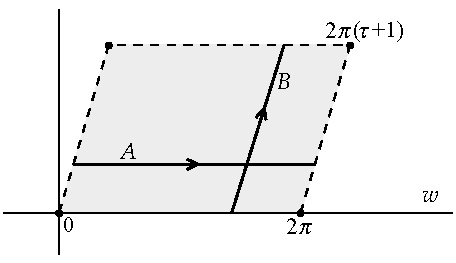
\includegraphics[width=0.8\linewidth]{figures/fig_5_1.pdf}
\caption{ゲージ $ds^2=dw\,d\bar w$ での、モジュラス $\tau$ をもつトーラス。上下の辺が同一視され、同様に左右の辺も同一視される。閉曲線 $A,B$ は、後で参照するために示してある。}
\label{fig:5.1}
\end{figure}

これを見るため、3.3節の局所的な議論で用いた手順を繰り返す。まず $2\nabla^2\omega=R$ を満たす Weyl 変換によって、計量を平坦にできる。$\nabla^2$ の固有モードで展開すると、周期境界条件の下では、$\omega$ に定数を加える自由を除いて一意な解が存在することがわかる。ここでは、Euler 数の $4\pi$ 倍である $\int d^2\sigma\,g^{1/2}R$ が、トーラスではゼロになることが重要である。続いて新しい座標 $\tilde\sigma^a$ に変換すれば、計量を単位計量の形にできる。しかし、点粒子の場合と同様、これが元の周期性を保つ保証はない。むしろ、今度は一般の並進 $u^a,v^a$ に対して、
\begin{equation}
\tilde\sigma^a\cong\tilde\sigma^a+2\pi(mu^a+nv^a)
\tag{5.1.10}\label{eq:5.1.10}
\end{equation}
となりうる。座標系を回転し、スケールを変え、それと同時に、計量の規格化を保つため $\omega$ をずらすことで、常に $u=(1,0)$ とおける。すると、$v$ の二つの成分という二つのパラメータが残る。$w=\tilde\sigma^1+i\tilde\sigma^2$ と定義すると、計量は $dw\,d\bar w$ で、周期性は
\begin{equation}
w\cong w+2\pi(m+n\tau)
\tag{5.1.11}\label{eq:5.1.11}
\end{equation}
となる。ここで $\tau=v^1+iv^2$ である。トーラスは、図\hyperref[fig:5.1]{5.1}に示すような、周期境界条件をもつ $w$ 平面内の平行四辺形である。

別の方法として、$w=\sigma^1+\tau\sigma^2$ によって $\sigma^a$ を定義しよう。元の周期性\hyperref[eq:5.1.8]{(5.1.8)}は保たれるが、計量は今度は、より一般的な形\hyperref[eq:5.1.9]{(5.1.9)}をとる。計量についての積分は、$\tau$ の実部と虚部についての二つの通常の積分に帰着する。計量\hyperref[eq:5.1.9]{(5.1.9)}は $\tau$ の複素共役に対して不変であり、$\tau$ が実数のとき退化するため、$\operatorname{Im}\tau>0$ に注意を限ることができる。円の\hyperref[eq:5.1.5a]{(5.1.5)}の場合と同様、これらのパラメータは、計量\hyperref[eq:5.1.9]{(5.1.9)}にも周期性\hyperref[eq:5.1.11]{(5.1.11)}にも入れられる。パラメータ $\tau$ は Teichmüller パラメータ、より一般的にはモジュラスと呼ばれる。点粒子の場合と異なるのは、円の不変な長さに類する、$\tau$ の簡単な不変表式がないことである。

点粒子の場合には対応物のない、追加の冗長性がいくらかある。$\tau+1$ という値は、$(m,n)\to(m-n,n)$ と置き換えることで、$\tau$ と同じ同一視の集合\hyperref[eq:5.1.11]{(5.1.11)}を生成する。$-1/\tau$ も、$w'=\tau w$ と定義して $(m,n)\to(n,-m)$ と置き換えれば同様である。これら二つの変換
\begin{equation}
T:\ \tau'=\tau+1,\qquad S:\ \tau'=-1/\tau
\tag{5.1.12}\label{eq:5.1.12}
\end{equation}
を繰り返し適用すると、$ad-bc=1$ を満たす任意の整数 $a,b,c,d$ に対する
\begin{equation}
\tau'=\frac{a\tau+b}{c\tau+d}
\tag{5.1.13}\label{eq:5.1.13}
\end{equation}
が生成される。

これは、次のようにも考えられる。変換
\begin{equation}
\begin{bmatrix}\sigma^1\\ \sigma^2\end{bmatrix}
=\begin{bmatrix}d&b\\c&a\end{bmatrix}
\begin{bmatrix}\sigma'^1\\ \sigma'^2\end{bmatrix}
\tag{5.1.14}\label{eq:5.1.14}
\end{equation}
は、$\sigma$ における計量\hyperref[eq:5.1.9]{(5.1.9)}を、$\sigma'$ における同じ形で、モジュラスが $\tau'$ となる計量に移す。これはトーラスの微分同相変換である。$ad-bc=1$ の帰結として一対一であり、周期性\hyperref[eq:5.1.8]{(5.1.8)}を保つ。しかし、無限小変換を順次行うことによって恒等変換から得ることはできない。いわゆる大きな座標変換である。座標 $\sigma$ での曲線 $A$ は、座標 $\sigma'$ では $A'$ 方向に $a$ 回、$B'$ 方向に $-c$ 回巡る曲線へ写る。これらの大きな座標変換は、行列式1の整数値 $2\times2$ 行列からなる群 $SL(2,\mathbb Z)$ をなす。$\tau$ 平面上の群は $SL(2,\mathbb Z)/\mathbb Z_2=PSL(2,\mathbb Z)$ である。$a,b,c,d$ の符号をすべて逆にしても、$\tau'$ は変わらないからである。変換\hyperref[eq:5.1.14]{(5.1.14)}の群は、モジュラー群と呼ばれる。

モジュラー変換\hyperref[eq:5.1.13]{(5.1.13)}を用いると、任意の $\tau$ が、図\hyperref[fig:5.2]{5.2}に示す領域 $F_0$、
\begin{equation}
-\frac12\leq\operatorname{Re}\tau\leq\frac12,\qquad |\tau|\geq1
\tag{5.1.15}\label{eq:5.1.15}
\end{equation}
の中のちょうど一点と等価であることを示せる。ただし、図のように同一視される境界は例外である。これは、上半平面を $PSL(2,\mathbb Z)$ で割った空間の基本領域と呼ばれる。同一視があるため、$F_0$ は巻き上げられ、$\operatorname{Im}\tau\to\infty$ のところだけが開いていると考えるべきである。基本領域 $F_0$ は、$(\mathrm{diff}\times\mathrm{Weyl})$ 非等価な計量のモジュライ空間の一つの表示である。

\begin{figure}[htbp]
\centering
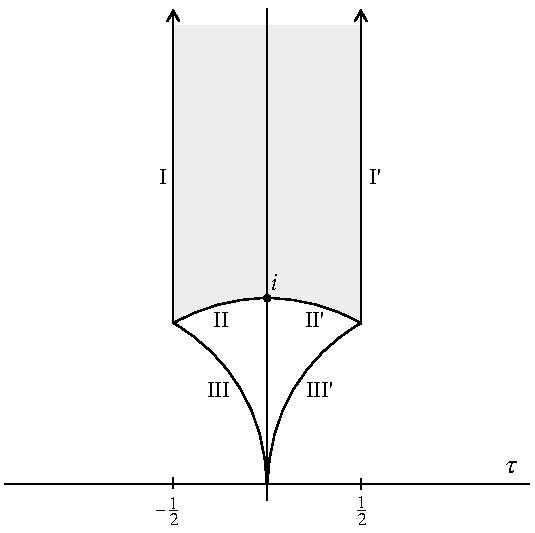
\includegraphics[width=0.8\linewidth]{figures/fig_5_2.pdf}
\caption{トーラスのモジュライ空間の標準的な基本領域 $F_0$。陰を付けて示してある。直線 I と I$'$ が同一視され、弧 II と II$'$ も同一視される。II、II$'$、III、III$'$ に囲まれた別の基本領域は、モジュラー変換 $S$ によって $F_0$ へ写される。}
\label{fig:5.2}
\end{figure}

点粒子の場合と同様、さらに厄介な点がある。$\tau$ が与えられた基本領域内にあり、計量が\hyperref[eq:5.1.9]{(5.1.9)}の形になることを要求しても、$\mathrm{diff}\times\mathrm{Weyl}$ 不変性のすべては固定されない。計量と周期性は、一様な並進
\begin{equation}
\sigma^a\longrightarrow\sigma^a+v^a
\tag{5.1.16}\label{eq:5.1.16}
\end{equation}
によって不変に保たれるので、$\mathrm{diff}\times\mathrm{Weyl}$ のこの二パラメータ部分群は固定されない。さらに、離散変換 $\sigma^a\to-\sigma^a$ も計量を不変にし、向き付けのない場合には、$\tau\to-\bar\tau$ を伴う $(\sigma^1,\sigma^2)\to(-\sigma^1,\sigma^2)$ もそうである。したがって、ここでも計量の自由度と局所対称性の間に二種類の不一致がある。対称性で取り除けない計量のパラメータと、計量の選択によって固定されない対称性である。固定されずに残る対称性は、共形 Killing 群（CKG）と呼ばれる。

振幅に十分な数の頂点演算子があれば、頂点演算子の位置のいくつかを固定することで、ゲージ不変性を完全に固定できる。$n$ 個の頂点演算子をもつトーラスでは、不変性\hyperref[eq:5.1.16]{(5.1.16)}を使って一つの頂点演算子の位置を固定でき、$\tau$ と残り $n-1$ 個の位置についての積分が残る。$\sigma^a\to-\sigma^a$ に由来する $\mathbb Z_2$ は、第二の頂点演算子をトーラスの半分に制限すれば固定できる。実際には、有限の重複計数については、一部の対称性を固定せずに残し、適切な因子で割る方が便利なことが多い。また、頂点演算子の数が少なすぎると、共形 Killing 不変性の一部が固定されずに残るので、その重複計数を明示的に考慮しなければならない。

\subsubsectionlink*{読者への注意}

この章の残りでは、モジュライをより一般的に論じ、ゲージ固定した積分の測度を求める。主な目標は、弦の $S$ 行列のゲージ固定した表式\hyperref[eq:5.3.9]{(5.3.9)}である。実際、弦の興味深い物理の大部分は、木のレベルと1ループの振幅で見ることができる。これらについては、近道を用いて測度を得られる。木のレベルの振幅には計量のモジュライはないが、いくつかの頂点演算子の位置を固定しなければならない。その測度は、式(6.4.4)の後で説明するように推定できる。1ループ振幅の測度は、式(7.3.9)の後の点粒子の測度の議論との類推から、かなり直観的に理解できる。したがって、読者はこの章の残りを飛ばしてもよい（あるいは、式\hyperref[eq:5.3.9]{(5.3.9)}までざっと読んでもよい）。また、Faddeev--Popov ゴーストを扱うすべての節を飛ばすこともできる。

\subsectionlink{モジュライとRiemann面}\label{sec:5.2}

前の議論を、より一般的かつ抽象的な形で繰り返そう。与えられた位相型 $r$ 上のすべての計量についての積分から出発する。計量の空間を $\mathcal G_r$ と呼ぶ。向き付けられた閉曲面では、$r$ は取っ手の数、すなわち種数 $g$ だけで指定できる。$\mathrm{diff}\times\mathrm{Weyl}$ の冗長性を考慮すると、モジュライ空間
\begin{equation}
\mathcal M_r=\frac{\mathcal G_r}{(\mathrm{diff}\times\mathrm{Weyl})_r}
\tag{5.2.1}\label{eq:5.2.1}
\end{equation}
が残る。トーラスの場合と同様、この空間は有限個のモジュライによってパラメータ付けられる。トーラスでは、$\mathcal M_1$ は上半平面を $PSL(2,\mathbb Z)$ で割った空間、あるいは等価的に、$F_0$ など任意の基本領域である。また、計量を不変にする $\mathrm{diff}\times\mathrm{Weyl}$ の部分群 CKG が存在する場合もある。

経路積分に頂点演算子があるときには、その位置を計量に由来するモジュライと同等に扱い、すべてをモジュライと呼ぶと便利である。区別が必要なときには、計量のモジュライと明示する。経路積分に頂点演算子がある場合に使える、CKG への対処法の一つは、一部の頂点演算子の座標を固定してゲージをさらに指定することである。Polyakov 経路積分には、$\mathcal G_r$ 上の積分と、$n$ 個の頂点演算子の位置を世界面 $M$ 上で積分するものが含まれる。したがって、位相型 $r$ で $n$ 個の頂点演算子をもつ場合のモジュライ空間は
\begin{equation}
\mathcal M_{r,n}
=\frac{\mathcal G_r\times M^n}{(\mathrm{diff}\times\mathrm{Weyl})_r}
\tag{5.2.2}\label{eq:5.2.2}
\end{equation}
である。

トーラスについて見たように、$\mathrm{diff}_r$ は一般には連結でない。恒等変換を含む連結成分 $\mathrm{diff}_{r0}$ を取り出すと、商
\begin{equation}
\frac{\mathrm{diff}_r}{\mathrm{diff}_{r0}}
\tag{5.2.3}\label{eq:5.2.3}
\end{equation}
がモジュラー群である。

計量の $\mathrm{diff}\times\mathrm{Weyl}$ 冗長性を無限小の水準で調べると興味深い。すなわち、$\mathrm{diff}\times\mathrm{Weyl}$ 変換と等価でなく、したがってモジュライの変化に対応する、小さな計量の変分を探す。また、計量を変えない小さな $\mathrm{diff}\times\mathrm{Weyl}$ 変換も探す。これらは CKG の無限小要素であり、共形 Killing ベクトル（CKV）と呼ばれる。このことから、モジュライと CKG の起源をさらに理解できる。

無限小 $\mathrm{diff}\times\mathrm{Weyl}$ 変換は、計量を
\begin{equation}
\delta g_{ab}=-2(P_1\delta\sigma)_{ab}
+(2\delta\omega-\nabla\cdot\delta\sigma)g_{ab}
\tag{5.2.4}\label{eq:5.2.4}
\end{equation}
だけ変える。ここで $P_1$ は、微分のトレースレスな対称線形結合(3.3.17)である。モジュライは、すべての変分\hyperref[eq:5.2.4]{(5.2.4)}に直交する計量の変分 $\delta'g_{ab}$ に対応する。
\begin{equation}
\begin{aligned}
0&=\int d^2\sigma\,g^{1/2}\delta'g_{ab}
\left[-2(P_1\delta\sigma)^{ab}
+(2\delta\omega-\nabla\cdot\delta\sigma)g^{ab}\right]\\
&=\int d^2\sigma\,g^{1/2}
\left[-2(P_1^T\delta'g)_a\delta\sigma^a
+\delta'g_{ab}g^{ab}(2\delta\omega-\nabla\cdot\delta\sigma)\right].
\end{aligned}
\tag{5.2.5}\label{eq:5.2.5}
\end{equation}
転置 $(P_1^Tu)_a=-\nabla^bu_{ab}$ は、演習3.2と同じように定義する。一般の $\delta\omega,\delta\sigma$ に対して内積\hyperref[eq:5.2.5]{(5.2.5)}がゼロになるには、
\begin{align}
g^{ab}\delta'g_{ab}&=0,
\tag{5.2.6a}\label{eq:5.2.6a}\\
(P_1^T\delta'g)_a&=0
\tag{5.2.6b}\label{eq:5.2.6b}
\end{align}
が必要である。第一の条件は、$\delta'g_{ab}$ のトレースがゼロであることを要求する。$P_1^T$ が作用するのは、このトレースレス対称テンソルである。これらの方程式の各解に対して、一つのモジュラスが存在する。

CKV は、$\delta g_{ab}=0$ となる変換\hyperref[eq:5.2.4]{(5.2.4)}である。この方程式のトレースは $\delta\omega$ を一意に固定し、共形 Killing 方程式
\begin{equation}
(P_1\delta\sigma)_{ab}=0
\tag{5.2.7}\label{eq:5.2.7}
\end{equation}
が残る。

共形ゲージの周りの変分に対しては、式\hyperref[eq:5.2.6a]{(5.2.6)}と\hyperref[eq:5.2.7]{(5.2.7)}は簡単になる。
\begin{align}
\partial_{\bar z}\delta'g_{zz}
&=\partial_z\delta'g_{\bar z\bar z}=0,
\tag{5.2.8a}\label{eq:5.2.8a}\\
\partial_{\bar z}\delta z&=\partial_z\delta\bar z=0.
\tag{5.2.8b}\label{eq:5.2.8b}
\end{align}
したがって、モジュライの変分は正則二次微分に、CKV は正則ベクトル場に対応する。トーラス上で正則かつ二重周期的な関数は定数だけなので、実モジュライが二つ、実 CKV が二つあり、前節の議論と一致する。

計量のモジュライは $P_1^T$ の核\hyperref[eq:5.2.6a]{(5.2.6)}に、CKV は $P_1$ の核\hyperref[eq:5.2.7]{(5.2.7)}に対応する。Riemann--Roch の定理は、計量のモジュライの数 $\mu=\dim\ker P_1^T$ と CKV の数 $\kappa=\dim\ker P_1$ を、Euler 数 $\chi$ に関係づける。
\begin{equation}
\mu-\kappa=-3\chi.
\tag{5.2.9}\label{eq:5.2.9}
\end{equation}
これは、この章の後で導くことができる。向き付けられた閉曲面では、$-3\chi=6g-6$ である。この数え方は実モジュライについてのものであり、$\tau$ のような複素モジュラスは実部と虚部に分けて数える。

さらに、$\chi<0$ では $\kappa$ がゼロとなり、$\chi>0$ では $\mu$ がゼロとなる。これを示すため、まず、Weyl 変換によってスカラー曲率 $R$ が一定になる計量を常に見いだせるという事実を用いる。このとき、$R$ の符号は $\chi$ の符号と同じである。$P_1^TP_1=-\tfrac12\nabla^2-\tfrac14R$ なので、
\begin{equation}
\begin{aligned}
\int d^2\sigma\,g^{1/2}
(P_1\delta\sigma)_{ab}(P_1\delta\sigma)^{ab}
&=\int d^2\sigma\,g^{1/2}
\delta\sigma_a(P_1^TP_1\delta\sigma)^a\\
&=\int d^2\sigma\,g^{1/2}
\left(\frac12\nabla_a\delta\sigma_b\nabla^a\delta\sigma^b
-\frac R4\delta\sigma_a\delta\sigma^a\right).
\end{aligned}
\tag{5.2.10}\label{eq:5.2.10}
\end{equation}
$\chi$ が負の場合、右辺は厳密に正なので、$P_1\delta\sigma$ はゼロになれない。同様の議論によって、$\chi$ が正の場合には $P_1^T\delta'g$ がゼロになれないことが示される。これらの結果を組み合わせると、
\begin{align}
\chi>0:&\qquad \kappa=3\chi,\quad\mu=0,
\tag{5.2.11a}\label{eq:5.2.11a}\\
\chi<0:&\qquad \kappa=0,\quad\mu=-3\chi
\tag{5.2.11b}\label{eq:5.2.11b}
\end{align}
を得る。

\subsubsectionlink*{Riemann面}

モジュライ空間を記述する馴染み深い方法は、各同値類から一つの計量を選ぶことである。これは、モジュライ $t^k$ に依存する計量の族 $\hat g_{ab}(t;\sigma)$ となる。トーラスでは、式\hyperref[eq:5.1.9]{(5.1.9)}がそのような切片を与える。計量 $dw\,d\bar w$ を固定し、モジュライを座標領域に組み込む\hyperref[eq:5.1.11]{(5.1.11)}の形の別の記述を用いると、しばしば便利である。この考えは、次のように形式化できる。

まず、可微分多様体の定義を思い出そう。多様体を、互いに重なり合うパッチの集合で覆い、第 $m$ パッチには座標 $\sigma_m^a$ を与える。$a$ は1から多様体の次元までの値をとる。パッチ $m,n$ が重なるとき、その二つのパッチの座標は
\begin{equation}
\sigma_m^a=f_{mn}^a(\sigma_n)
\tag{5.2.12}\label{eq:5.2.12}
\end{equation}
によって関係づけられ、遷移関数 $f_{mn}$ には、指定された回数だけ微分可能であることを要求する。Riemann 多様体では、各パッチに計量 $g_{m,ab}(\sigma_m)$ も与えられ、重なりでの値は通常のテンソル変換則によって関係づけられる。

複素多様体では、各パッチに複素座標 $z_m^a$ があり、今度は $a$ が1から多様体の次元の半分まで動く。遷移関数は正則であることを要求する。
\begin{equation}
z_m^a=f_{mn}^a(z_n).
\tag{5.2.13}\label{eq:5.2.13}
\end{equation}
正則性はどの座標 $z_m^a$ を使うかに依存しないので、多様体上の正則関数を定義できる。二つの可微分多様体の間に一対一の可微分写像があればそれらが等価であるのと同様に、二つの複素多様体の間に一対一の正則写像があれば、それらは等価である。とくに、各パッチの内部で正則な座標変換を行うと、等価な曲面が得られる。

二次元、すなわち複素座標が一つの場合、複素多様体は Riemann面と呼ばれる。この場合、一対一対応
\begin{equation}
\text{Riemann面}\quad\longleftrightarrow\quad
\text{Riemann 多様体を Weyl 変換で割ったもの}
\tag{5.2.14}\label{eq:5.2.14}
\end{equation}
がある。右辺で「Weyl 変換で割る」とだけしたのは、「微分同相変換で割る」ことがすでに Riemann 多様体の定義に暗黙に含まれるからである。この同型を見るため、Riemann 多様体から出発しよう。共形ゲージの議論から、各座標パッチ内に、
\begin{equation}
ds^2\propto dz_m\,d\bar z_m
\tag{5.2.15}\label{eq:5.2.15}
\end{equation}
を満たす座標 $z_m$ を見つけられることがわかっている。隣接するパッチでは座標が同じである必要はないが、$ds^2\propto dz_m\,d\bar z_m\propto dz_n\,d\bar z_n$ なので、遷移関数は正則となる。\footnote[1]{正確には、反正則な遷移関数も可能である。向き付けられた弦では、標準の向きを選ぶことでこれを禁止する。向き付けのない弦では許される。厳密な意味での Riemann面は、境界をもたない向き付けられた多様体を指す。}
これが、実二次元における Riemann 多様体から複素多様体への写像である。逆写像については、第 $m$ パッチの計量を $dz_m\,d\bar z_m$ とし、重なりで滑らかにつなぐことで（これは1の分割という標準的な構成である）、Riemann 多様体を作れる。したがって、Riemann面の二つの特徴づけは等価である。

平行四辺形（図\hyperref[fig:5.1]{5.1}）の複素座標 $w$ によるトーラスの記述は、複素多様体という考えを具体的に示している。図\hyperref[fig:5.1]{5.1}の基本平行四辺形より少し大きい一つの座標パッチをとると考えよう。周期性の条件
\begin{equation}
w\cong w+2\pi\cong w+2\pi\tau
\tag{5.2.16}\label{eq:5.2.16}
\end{equation}
は、そのパッチの向かい合う辺の重なりにおける遷移関数となる。曲面は、これらの遷移関数によって定義される。元の計量についての経路積分を定義するには、まず計量を、正方形\hyperref[eq:5.1.7]{(5.1.7)}のような固定座標上の関数、あるいは少なくとも、固定した遷移関数をもつ固定した座標パッチの集合上の関数とみなすのが最も簡単である。その後、与えられた曲面上の場の量子論を調べるには、平行四辺形\hyperref[eq:5.1.11]{(5.1.11)}のように、単位計量と、モジュライに依存する遷移関数を用いるのが最も容易である。

Riemann面は、次のようにも考えられる。世界面をパッチの和集合として定義し、$\mathrm{diff}\times\mathrm{Weyl}$ の自由を用いて、各パッチで計量を $dz\,d\bar z$ にできる。すると、重なり合うパッチでのゲージの選択は、この計量を不変にする $\mathrm{diff}\times\mathrm{Weyl}$ 変換によってのみ異なりうる。すでに議論したように、これらは共形変換である。したがって Riemann面は、CFT が定義される自然な場所である。CFT の場は、共形変換の下で確定した変換性をもつからである。

\subsectionlink{モジュライの測度}\label{sec:5.3}

ここで、Polyakov 経路積分のゲージ固定を再び考える。ゲージ冗長性は、計量についての経路積分を完全には取り除かず、モジュライ空間上の有限次元積分を残すことを学んだ。これを考慮するために、3.3節の議論を精密化する必要がある。

$S$ 行列の Polyakov 経路積分は
\begin{equation}
\begin{aligned}
S_{j_1\cdots j_n}(k_1,\ldots,k_n)
={}&\sum_{\substack{\text{コンパクトな}\\\text{位相型}}}
\int\frac{[d\phi\,dg]}{V_{\mathrm{diff}\times\mathrm{Weyl}}}
\exp(-S_{\mathrm m}-\lambda\chi)\\
&\quad\times\prod_{i=1}^n
\int d^2\sigma_i\,g(\sigma_i)^{1/2}
\mathcal V_{j_i}(k_i,\sigma_i)
\end{aligned}
\tag{5.3.1}\label{eq:5.3.1}
\end{equation}
である。これは以前の表式\hyperref[eq:3.5.5]{(3.5.5)}だが、今度は一般の $c=\tilde c=26$ の物質理論を用いて書き、物質場を $\phi$ と表している。ゲージ固定では、計量と位置についての積分を、ゲージ群、モジュライ、固定されていない位置についての積分に変換する。
\begin{equation}
[dg]\,d^{2n}\sigma\longrightarrow[d\zeta]\,d^\mu t\,d^{2n-\kappa}\sigma.
\tag{5.3.2}\label{eq:5.3.2}
\end{equation}
ゲージ群の体積を分離して除いた後、この変換の Jacobian がモジュライ空間上の測度となる。

手順は3.3節と同じだが、今度はモジュライと CKV を考慮する。とくに、ゲージの選択は、頂点演算子の座標のうち $\kappa$ 個を $\sigma_i^a\to\hat\sigma_i^a$ と固定することになる。固定された座標 $(a,i)$ の集合を $f$ と表す。モジュライ空間上の Faddeev--Popov 測度を
\begin{equation}
1=\Delta_{\mathrm{FP}}(g,\sigma)
\int_Fd^\mu t\int_{\mathrm{diff}\times\mathrm{Weyl}}[d\zeta]\,
\delta\bigl(g-\hat g(t)^\zeta\bigr)
\prod_{(a,i)\in f}\delta\bigl(\sigma_i^a-\hat\sigma_i^{\zeta a}\bigr)
\tag{5.3.3}\label{eq:5.3.3}
\end{equation}
によって定義する。定義により、すべての計量は、少なくとも一組の $t,\zeta$ の値について $\hat g(t)$ と $(\mathrm{diff}\times\mathrm{Weyl})$ 等価である。固定座標のデルタ関数は、そこから一意の $\zeta$ を選び出す。ただし、5.1節の最後で述べたように、位数が有限の $n_R$ である離散対称群が残る場合がある。その場合、デルタ関数は $n_R$ 個の点でゼロでなくなる。

表式\hyperref[eq:5.3.3]{(5.3.3)}を経路積分\hyperref[eq:5.3.1]{(5.3.1)}に挿入し、以前と同じ手順を踏むと、
\begin{equation}
\begin{aligned}
S_{j_1\cdots j_n}(k_1,\ldots,k_n)
={}&\sum_{\substack{\text{コンパクトな}\\\text{位相型}}}
\int_Fd^\mu t\,\Delta_{\mathrm{FP}}\bigl(\hat g(t),\hat\sigma\bigr)
\int[d\phi]\int\prod_{(a,i)\notin f}d\sigma_i^a\\
&\quad\times\exp\bigl(-S_{\mathrm m}[\phi,\hat g(t)]-\lambda\chi\bigr)
\prod_{i=1}^n\left[\hat g(\sigma_i)^{1/2}
\mathcal V_{j_i}(k_i;\sigma_i)\right]
\end{aligned}
\tag{5.3.4}\label{eq:5.3.4}
\end{equation}
を得る。計量と頂点演算子の座標についての積分は、計量のモジュライ空間 $F$ と固定されていない座標についての積分に帰着し、その測度は $\Delta_{\mathrm{FP}}$ によって与えられている。頂点演算子では、位置のうち $\kappa$ 個が固定されている。

次に、Faddeev--Popov 測度を評価する。デルタ関数は、対称性で関係づけられた $n_R$ 個の点でゼロでないため、そのうちの一点を考え、$n_R$ で割る。その点の近くで、$\Delta_{\mathrm{FP}}$ の定義\hyperref[eq:5.3.3]{(5.3.3)}を展開する。一般の計量の変分は、局所対称変換による変分とモジュライ $t^k$ の変化との和に等しい。
\begin{equation}
\delta g_{ab}
=\sum_{k=1}^{\mu}\delta t^k\partial_{t^k}\hat g_{ab}
-2(\hat P_1\delta\sigma)_{ab}
+(2\delta\omega-\hat\nabla\cdot\delta\sigma)\hat g_{ab}.
\tag{5.3.5}\label{eq:5.3.5}
\end{equation}
すると、Faddeev--Popov 行列式の逆数は
\begin{equation}
\begin{aligned}
\Delta_{\mathrm{FP}}(\hat g,\hat\sigma)^{-1}
&=n_R\int d^\mu\delta t\,[d\delta\omega\,d\delta\sigma]\,
\delta(\delta g_{ab})
\prod_{(a,i)\in f}\delta\bigl(\delta\sigma^a(\hat\sigma_i)\bigr)\\
&=n_R\int d^\mu\delta t\,d^\kappa x\,[d\beta'\,d\delta\sigma]\\
&\quad\times\exp\left[
2\pi i(\beta',2\hat P_1\delta\sigma-\delta t^k\partial_k\hat g)
+2\pi i\sum_{(a,i)\in f}x_{ai}\delta\sigma^a(\hat\sigma_i)
\right].
\end{aligned}
\tag{5.3.6}\label{eq:5.3.6}
\end{equation}
第二の表式の内積は、演習3.2で定義したものである。3.3節の局所的な議論と同じ手順に従い、デルタ関数とデルタ汎関数を $x$ と $\beta_{ab}$ の積分として書き、その後 $\delta\omega$ を積分して、$\beta'_{ab}$ のトレースがゼロであるという制約を得た。

以前と同じく、すべてのボソン変数を Grassmann 変数に置き換えることで、積分\hyperref[eq:5.3.6]{(5.3.6)}の逆数をとる。
\begin{align}
\delta\sigma^a&\longrightarrow c^a,
\tag{5.3.7a}\label{eq:5.3.7a}\\
\beta'_{ab}&\longrightarrow b_{ab},
\tag{5.3.7b}\label{eq:5.3.7b}\\
x_{ai}&\longrightarrow\eta_{ai},
\tag{5.3.7c}\label{eq:5.3.7c}\\
\delta t^k&\longrightarrow\xi^k.
\tag{5.3.7d}\label{eq:5.3.7d}
\end{align}
すると、場を便利に規格化すれば、
\begin{equation}
\begin{aligned}
\Delta_{\mathrm{FP}}(\hat g,\hat\sigma)
&=\frac1{n_R}\int[db\,dc]\,d^\mu\xi\,d^\kappa\eta\\
&\quad\times\exp\left[
-\frac1{4\pi}(b,2\hat P_1c-\xi^k\partial_k\hat g)
+\sum_{(a,i)\in f}\eta_{ai}c^a(\hat\sigma_i)\right]\\
&=\frac1{n_R}\int[db\,dc]\exp(-S_{\mathrm g})
\prod_{k=1}^{\mu}\frac1{4\pi}(b,\partial_k\hat g)
\prod_{(a,i)\in f}c^a(\hat\sigma_i).
\end{aligned}
\tag{5.3.8}\label{eq:5.3.8}
\end{equation}
最後の行では、Grassmann パラメータ $\eta_{ai},\xi^k$ を積分した。

モジュライ空間上の積分に適した測度は、挿入を伴うこのゴースト経路積分によって生成される。途中の段階で全体の符号を追跡することはしない。これは Jacobian であるべきものなので、正の結果を与えるように全体の符号を暗黙に選ぶ。その結果、$S$ 行列の完全な表式は
\begin{equation}
\begin{aligned}
S_{j_1\cdots j_n}(k_1,\ldots,k_n)
={}&\sum_{\substack{\text{コンパクトな}\\\text{位相型}}}
\int_F\frac{d^\mu t}{n_R}
\int[d\phi\,db\,dc]\exp(-S_{\mathrm m}-S_{\mathrm g}-\lambda\chi)\\
&\times\prod_{(a,i)\notin f}\int d\sigma_i^a\,
\prod_{k=1}^{\mu}\frac1{4\pi}(b,\partial_k\hat g)\\
&\times\prod_{(a,i)\in f}c^a(\hat\sigma_i)\,
\prod_{i=1}^n\hat g(\sigma_i)^{1/2}\mathcal V_{j_i}(k_i,\sigma_i)
\end{aligned}
\tag{5.3.9}\label{eq:5.3.9}
\end{equation}
となる。この結果は、閉弦と開弦、向き付けのあるものとないものという、すべてのボソン弦理論に容易に拡張できる。違いは、含まれる位相型と許される頂点演算子だけである。式\hyperref[eq:5.3.9]{(5.3.9)}は、有用で優美な結果である。モジュライと CKV に由来する複雑さは、経路積分の中の $c,b$ の挿入によって考慮される。固定座標ごとに $d\sigma_i^a$ が $c_i^a$ に置き換わり、各計量モジュラスは一つの $b$ の挿入を生じさせる。

\subsubsectionlink*{行列式による表式}

式\hyperref[eq:5.3.8]{(5.3.8)}では、Faddeev--Popov 行列式を、Grassmann パラメータと場についての積分で表した。ここでは、これを有限次元の行列式と汎関数行列式の積に帰着させる。後の章で弦の $S$ 行列を調べるとき、この直接的な経路積分によるアプローチは、用いる方法の一つとなる。

ゴースト場を適切な完全系で展開する。
\begin{equation}
c^a(\sigma)=\sum_Jc_JC_J^a(\sigma),\qquad
b_{ab}(\sigma)=\sum_Kb_KB_{Kab}(\sigma).
\tag{5.3.10}\label{eq:5.3.10}
\end{equation}
完全系 $C_J^a,B_{Kab}$ は、次のように定義する。ゴースト作用に現れる微分 $P_1$ は、ベクトルをトレースレス対称テンソルに移す。その転置は逆のことを行う。ゴースト作用は、どちらを用いても書ける。
\begin{equation}
S_{\mathrm g}=\frac1{2\pi}(b,P_1c)
=\frac1{2\pi}(P_1^Tb,c).
\tag{5.3.11}\label{eq:5.3.11}
\end{equation}
$P_1$ はある種類の場を別の種類の場に変えるため、微分同相不変な仕方で対角化することはできない。しかし、$P_1^TP_1$ と $P_1P_1^T$ は対角化できる。
\begin{equation}
P_1^TP_1C_J^a=\nu_J'^2C_J^a,\qquad
P_1P_1^TB_{Kab}=\nu_K^2B_{Kab}.
\tag{5.3.12}\label{eq:5.3.12}
\end{equation}
固有関数は実に選ぶことができ、それぞれの内積
\begin{align}
(C_J,C_{J'})
&=\int d^2\sigma\,g^{1/2}C_J^aC_{J'a}
=\delta_{JJ'},
\tag{5.3.13a}\label{eq:5.3.13a}\\
(B_K,B_{K'})
&=\int d^2\sigma\,g^{1/2}B_{Kab}B_{K'}^{ab}
=\delta_{KK'}
\tag{5.3.13b}\label{eq:5.3.13b}
\end{align}
によって規格化する。

ここで、
\begin{equation}
(P_1P_1^T)P_1C_J
=P_1(P_1^TP_1)C_J=\nu_J'^2P_1C_J
\tag{5.3.14}\label{eq:5.3.14}
\end{equation}
に注意しよう。したがって、$P_1C_J$ は $P_1P_1^T$ の固有関数である。同様に、$P_1^TB_K$ は $P_1^TP_1$ の固有関数である。よって、$P_1C_J=0$ または $P_1^TB_K=0$ の場合を除いて、固有関数の間には一対一対応がある。後者は、$P_1^TP_1$ または $P_1P_1^T$ のゼロ固有値に対応する。これらはまさに CKV と正則二次微分なので、その数はそれぞれ $\kappa,\mu$ である。固有値ゼロの固有関数は $C_{0j},B_{0k}$ と表し、ゼロでない固有値には $J,K=1,\ldots$ という添字を付けよう。後者については、規格化された固有関数の間に
\begin{equation}
B_{Jab}=\frac1{\nu_J}(P_1C_J)_{ab},\qquad
\nu_J=\nu'_J\ne0
\tag{5.3.15}\label{eq:5.3.15}
\end{equation}
という関係がある。

モードで書くと、ゴースト経路積分 $\Delta_{\mathrm{FP}}$ は
\begin{equation}
\begin{aligned}
&\int\prod_{k=1}^{\mu}db_{0k}
\prod_{j=1}^{\kappa}dc_{0j}
\prod_Jdb_J\,dc_J\,
\exp\left(-\frac{\nu_Jb_Jc_J}{2\pi}\right)\\
&\qquad\times\prod_{k'=1}^{\mu}\frac1{4\pi}(b,\partial_{k'}\hat g)
\prod_{(a,i)\in f}c^a(\sigma_i)
\end{aligned}
\tag{5.3.16}\label{eq:5.3.16}
\end{equation}
となる。A.2節によれば、Grassmann 積分は、積分変数が被積分関数に現れない限りゼロになる。$c_{0j},b_{0k}$ は作用には現れず、挿入の中にだけ現れる。実際、積分\hyperref[eq:5.3.16]{(5.3.16)}の中のそれぞれの種類の挿入の数 $\kappa,\mu$ は、対応するゴーストのゼロモードの数とちょうど一致する。ゼロでない答えを得るのに必要なだけの挿入がちょうどあり、挿入ではゴースト場のゼロモード部分だけが寄与する。したがって、
\begin{equation}
\begin{aligned}
\Delta_{\mathrm{FP}}
={}&\int\prod_{k=1}^{\mu}db_{0k}
\prod_{k'=1}^{\mu}\left[
\sum_{k''=1}^{\mu}\frac{b_{0k''}}{4\pi}
(B_{0k''},\partial_{k'}\hat g)\right]\\
&\times\int\prod_{j=1}^{\kappa}dc_{0j}
\prod_{(a,i)\in f}\left[
\sum_{j'=1}^{\kappa}c_{0j'}C_{0j'}^a(\sigma_i)\right]\\
&\times\int\prod_Jdb_J\,dc_J
\exp\left(-\frac{\nu_Jb_Jc_J}{2\pi}\right).
\end{aligned}
\tag{5.3.17}\label{eq:5.3.17}
\end{equation}
ゼロモード積分を Grassmann 変数で飽和させるすべての仕方について和をとると、それぞれで有限次元の行列式が生成される。一方、非ゼロモードは無限積、すなわち汎関数行列式を与える。全体として、
\begin{equation}
\Delta_{\mathrm{FP}}
=\det\frac{(B_{0k},\partial_{k'}\hat g)}{4\pi}\,
\det C_{0j}^a(\sigma_i)\,
\left[\det{}'\left(\frac{P_1^TP_1}{4\pi^2}\right)\right]^{1/2}.
\tag{5.3.18}\label{eq:5.3.18}
\end{equation}
$C_{0j}^a(\sigma_i)$ が正方行列であることに注意しよう。$(a,i)\in f$ がとる値は、$j$ と同じく $\kappa$ 個である。汎関数行列式のプライムは、ゼロ固有値を除くことを表す。

\subsubsectionlink*{Riemann--Roch の定理}

これで、Riemann--Roch の定理を経路積分から導くことができる。正則な $bc$ 系（$\tilde b,\tilde c$ を含まない）のゴーストカレントについて、演習3.6で導いたカレント保存則の異常は
\begin{equation}
\nabla_aj^a=\frac{1-2\lambda}{4}R
\tag{5.3.19}\label{eq:5.3.19}
\end{equation}
である。

Noether の定理は、保存カレントを不変性に関係づける。保存しないカレントについても同じ議論を行うと、
\begin{equation}
\frac{\delta\bigl([d\phi]\exp(-S)\bigr)}
{[d\phi]\exp(-S)}
=\frac{i\epsilon}{2\pi}\int d^2\sigma\,g^{1/2}\nabla_aj^a
\longrightarrow-i\epsilon\frac{2\lambda-1}{2}\chi
\tag{5.3.20}\label{eq:5.3.20}
\end{equation}
が得られる。ゴースト数の対称性は $\delta b=-i\epsilon b$、$\delta c=i\epsilon c$ と作用する。経路積分がゼロでないとき、測度、作用、挿入の変換は相殺しなければならない。したがって、異常から、$c$ の挿入の数から $b$ の挿入の数を引いたものは $3\chi/2$ であるとわかる。経路積分の計算は、挿入の数をゼロモードの数に関係づけるので、同じ差に対して
\begin{equation}
\frac12(\kappa-\mu)
=\frac12(\dim\ker P_1-\dim\ker P_1^T)
\tag{5.3.21}\label{eq:5.3.21}
\end{equation}
を与える。因子 $\tfrac12$ が現れるのは、正則な理論だけをとったからである。反正則な理論は同じ寄与を与える。異常から得た結果とゼロモードから得た結果を等置すれば、Riemann--Roch の定理 $\kappa-\mu=3\chi$ が得られる。一般の $bc$ 系についても、同じように
\begin{equation}
\dim\ker P_n-\dim\ker P_n^T=(2n+1)\chi
\tag{5.3.22}\label{eq:5.3.22}
\end{equation}
が得られる。これらの演算子は演習3.2で定義されている。

\subsectionlink{測度についての補足}

ここでは、ゲージ固定した弦の振幅の一般的な性質をいくつかまとめる。これらは主として、第9章の、より形式的な考察に役立つ。

\subsubsectionlink*{ゲージ不変性}

Faddeev--Popov の手続きによって、ゲージ固定した振幅が BRST 不変であり、ゲージの選び方に依存しないことは保証されている。しかし、期待される不変性をすべて備えていることを明示的に確かめておくのは有用である。第一に、振幅はモジュライ空間上の座標 $t$ の選び方に依存しない。新しい座標 $t'{}^k(t)$ に対して、
\begin{equation}
\begin{aligned}
d^\mu t'&=\left|\det\frac{\partial t'}{\partial t}\right|d^\mu t,\\
\prod_{k=1}^{\mu}\frac{1}{4\pi}(b,\partial'_k\hat g)
&=\det\left(\frac{\partial t}{\partial t'}\right)
\prod_{k=1}^{\mu}\frac{1}{4\pi}(b,\partial_k\hat g)
\end{aligned}
\tag{5.4.1}\label{eq:5.4.1}
\end{equation}
となり、二つの Jacobian は相殺する（符号を除く。この符号は、すでに述べたように、測度が正になるよう手で定めなければならない）。言い換えると、$b$ ゴーストの挿入によって、被積分関数はモジュライ空間上の密度として変換する。

第二に、測度がゲージ切片の Weyl 変換のもとで不変であることを見よう。Weyl 変換
\begin{equation}
\delta\hat g'_{ab}(t;\sigma)
=2\delta\omega(t;\sigma)\hat g_{ab}(t;\sigma)
\tag{5.4.2}\label{eq:5.4.2}
\end{equation}
のもとで、作用と測度の変分は局所演算子 $T^a{}_a$ の挿入を与える。これは $D=26$ では運動方程式によって消える。したがって、さまざまな挿入への影響だけを考えればよい。頂点演算子の挿入は、その構成から Weyl 不変である。$c^a(\sigma_i)$ の挿入は、式(3.3.24)の下で議論したように Weyl 不変である。$b$ の挿入については、
\begin{equation}
\begin{aligned}
(b,\partial_k\hat g')
&=\int d^2\sigma\,\hat g'{}^{1/2}b_{ab}
\hat g'{}^{ac}\hat g'{}^{bd}\partial_k\hat g'_{cd}\\
&=\int d^2\sigma\,\hat g^{1/2}b_{ab}
\left(\hat g^{ac}\hat g^{bd}\partial_k\hat g_{cd}
+2\hat g^{ab}\partial_k\omega\right)\\
&=(b,\partial_k\hat g)
\end{aligned}
\tag{5.4.3}\label{eq:5.4.3}
\end{equation}
であり、最後の等式は $b$ がトレースレスであることによる。

第三に、無限小の diff 変換 $\delta\sigma=\xi(t;\sigma)$ のもとでの不変性を確かめよう。一般の diff 変換への拡張は容易である。振幅\hyperref[eq:5.3.9]{(5.3.9)}のうち、不変性がただちには明らかでない項は、$b$ の挿入と、座標が固定された頂点演算子だけである。前者は
\begin{equation}
\begin{aligned}
\delta(b,\partial_k\hat g)
&=-2(b,P_1\partial_k\xi)\\
&=-2(P_1^Tb,\partial_k\xi)\\
&=0
\end{aligned}
\tag{5.4.4}\label{eq:5.4.4}
\end{equation}
と変換する。ここでは $b$ の運動方程式を用いた。$b$ の運動方程式は $\delta S/\delta c=0$ から得られるので、$c$ の挿入の位置には源の項が現れる。これらは、固定された頂点演算子への座標変換の影響を取り込むために、まさに必要なものである。

\subsubsectionlink*{BRST 不変性}

次に、振幅\hyperref[eq:5.3.9]{(5.3.9)}の完全な BRST 不変性を確かめる。経路積分の測度と作用が不変であることは局所的な解析からわかっているので、挿入に対する BRST 変換の影響を考える必要がある。ゲージ固定した経路積分\hyperref[eq:5.3.9]{(5.3.9)}では、積分しない頂点演算子には $c$ または $\tilde c c$ の因子が伴う。これは、OCQ 状態に対応する BRST 不変な頂点演算子について、第4.4節の末尾で述べたものにほかならない。一方、積分する頂点演算子は BRST 不変ではないが、その BRST 変分が
\begin{equation}
\delta_B\mathcal V_{\mathrm m}
=i\epsilon\,\partial_a(c^a\mathcal V_{\mathrm m})
\tag{5.4.5}\label{eq:5.4.5}
\end{equation}
であることを示すのは演習とする。これは積分すれば消える。

最後に、$b$ の挿入の変分がある。
\begin{equation}
\delta_B(b,\partial_k\hat g)=i\epsilon(T,\partial_k\hat g).
\tag{5.4.6}\label{eq:5.4.6}
\end{equation}
このエネルギー運動量テンソルの挿入は、ちょうどモジュラス $t^k$ に関する微分を生むので、BRST 変分は、モジュライ空間の境界からの項が生じる可能性を除けば消える。今後の章ではモジュライ空間の境界を調べる。ほとんどの場合、伝播関数の相殺の議論と呼ばれるものにより、表面からの寄与は存在しない。ある状況ではこの議論が適用できず、その場合の扱い方も見ていく。

ゲージ固定した結果\hyperref[eq:5.3.9]{(5.3.9)}は、ゲージ不変な形式を参照せず、BRST 不変性の要求から直接書き下すこともできる、という点に注意する必要がある。ゴースト経路積分を評価した際に見たように、少なくとも $\mu$ 個の $b$ の挿入と $\kappa$ 個の $c$ の挿入がなければ、経路積分は消える。振幅\hyperref[eq:5.3.9]{(5.3.9)}には、ゼロでない結果を与えるのにちょうど必要な数のゴーストが挿入されている。必要な $b$ の因子を含めると、BRST 変分によって、計量の $t^k$ 微分と畳み込まれたエネルギー運動量テンソルが現れる。これはモジュライに関する微分に比例するので、ここで行ったようにモジュライ空間上で積分して初めて、不変な結果が得られる。結果\hyperref[eq:5.3.9]{(5.3.9)}は、さまざまに一般化できる。たとえば、共形 Killing 不変性の一部を固定せずに残す場合がある。第7章では、頂点演算子を持たないトーラスの例について、これを明示的に示す。

BRST 不変性から、BRST 同値な状態に対する振幅は等しいことが従う。どの状態に対しても、ヌルな部分 $Q_B\lvert\chi\rangle$ を加えると、その効果は経路積分中に変分 $\delta_B\mathcal V_\chi$ を挿入することになり、これは積分するとゼロになる。物理的 Hilbert 空間はコホモロジーと同一視されるので、同値な状態は等しい振幅を持つはずであり、この性質は重要である。

\subsubsectionlink*{Riemann面の測度}

Faddeev--Popov 測度は、ゲージ固定した世界面を、モジュライに依存する計量で記述する枠組みで導いた。次に、この結果を、構造をモジュライに依存する遷移関数で表す Riemann面の枠組みに書き換える。

モジュライ空間のある点 $t_0$ で測度を表すために、$m$ 番目のパッチに複素座標 $z_m$ を持ち、遷移関数が正則である座標パッチの集合をとろう。各パッチで、計量 $\hat g(t_0)$ は $dz_m\,d\bar z_m$ と Weyl 同値である。ここで、モジュライの変化を考える。まず、遷移関数を固定したままでの計量の変化として記述し、次に、計量を固定したままでの遷移関数の変化に変換する。第一の記述では、Beltrami 微分
\begin{equation}
\mu_{ka}{}^b=\frac12\hat g^{bc}\partial_k\hat g_{ac}
\tag{5.4.7}\label{eq:5.4.7}
\end{equation}
を定義する。$\delta t^k$ に対する $b$ の挿入は
\begin{equation}
\frac{1}{2\pi}(b,\mu_k)
=\frac{1}{2\pi}\int d^2z\,
\left(b_{zz}\mu_{k\bar z}{}^z
+b_{\bar z\bar z}\mu_{kz}{}^{\bar z}\right)
\tag{5.4.8}\label{eq:5.4.8}
\end{equation}
となる。第二の記述では、モジュライを $\delta t^k$ だけ変えると、各パッチに新しい座標
\begin{equation}
z'_m=z_m+\delta t^k v_{km}^{z_m}(z_m,\bar z_m)
\tag{5.4.9}\label{eq:5.4.9}
\end{equation}
が現れる。$v_{km}^a$ の上付き添字はベクトル添字である。$v_{km}^a$ は $m$ 番目のパッチでのみ定義されていることに注意しよう。Riemann面の定義から、$dz'_m\,d\bar z'_m$ は $t_0+\delta t$ における計量と Weyl 同値である。
\begin{equation}
dz'_m\,d\bar z'_m
\propto dz_m\,d\bar z_m
+\delta t^k\left(
\mu_{kz_m}{}^{\bar z_m}\,dz_m\,dz_m
+\mu_{k\bar z_m}{}^{z_m}\,d\bar z_m\,d\bar z_m
\right).
\tag{5.4.10}\label{eq:5.4.10}
\end{equation}
したがって、座標変換 $v_{km}^a$ と Beltrami 微分は
\begin{equation}
\mu_{kz_m}{}^{\bar z_m}=\partial_{z_m}v_{km}^{\bar z_m},
\qquad
\mu_{k\bar z_m}{}^{z_m}=\partial_{\bar z_m}v_{km}^{z_m}
\tag{5.4.11}\label{eq:5.4.11}
\end{equation}
で関係づけられる。これは Beltrami 方程式の無限小版である。この式から $v_{km}^{z_m}$ は正則でないことがわかる。そうでなければ、モジュライの変化に対応しない。また、$v_{km}^{z_m}$ には Beltrami 方程式では決まらない正則な部分があり、$v_{km}^{\bar z_m}$ には反正則な部分がある。これらは、各パッチの内部で正則な再パラメータ化を行う自由度に対応する。

部分積分すると、$b$ の挿入\hyperref[eq:5.4.8]{(5.4.8)}は
\begin{equation}
\frac{1}{2\pi}(b,\mu_k)
=\frac{1}{2\pi i}\sum_m\oint_{C_m}
\left(dz_m\,v_{km}^{z_m}b_{z_mz_m}
-d\bar z_m\,v_{km}^{\bar z_m}b_{\bar z_m\bar z_m}\right)
\tag{5.4.12}\label{eq:5.4.12}
\end{equation}
となる。輪郭 $C_m$ は $m$ 番目のパッチを反時計回りに一周する。式\hyperref[eq:5.4.9]{(5.4.9)}より、ある点での座標のモジュライに関する微分は
\begin{equation}
\frac{dz_m}{dt^k}=v_{km}^{z_m}
\tag{5.4.13}\label{eq:5.4.13}
\end{equation}
である。したがって、モジュライの変化に伴う遷移関数の変化は
\begin{equation}
\left.\frac{\partial z_m}{\partial t^k}\right|_{z_n}
=v_{km}^{z_m}
-\left.\frac{\partial z_m}{\partial z_n}\right|_t v_{kn}^{z_n}
=v_{km}^{z_m}-v_{kn}^{z_m}
\tag{5.4.14}\label{eq:5.4.14}
\end{equation}
である。

\begin{figure}[tbp]
\centering
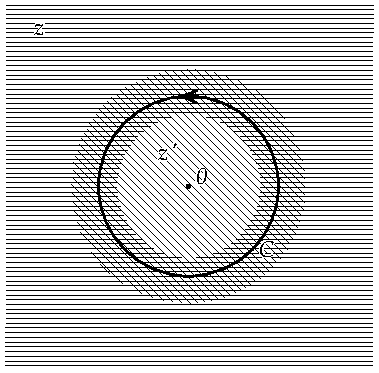
\includegraphics[width=0.8\linewidth]{figures/fig_5_3.pdf}
\caption{座標パッチ $z'$（斜線）と $z$（横線）。頂点演算子は $z'=0$ にある。環状領域では $z=z'+z_v$。}
\label{fig:5.3}
\end{figure}

隣り合うパッチの周りの輪郭積分\hyperref[eq:5.4.12]{(5.4.12)}を合わせると、
\begin{equation}
\begin{aligned}
\frac{1}{2\pi}(b,\mu_k)
=\frac{1}{2\pi i}\sum_{(mn)}\int_{C_{mn}}
\biggl[
&dz_m\,\left.\frac{\partial z_m}{\partial t^k}\right|_{z_n}
b_{z_mz_m}\\
&-d\bar z_m\,\left.\frac{\partial\bar z_m}{\partial t^k}\right|_{z_n}
b_{\bar z_m\bar z_m}
\biggr]
\end{aligned}
\tag{5.4.15}\label{eq:5.4.15}
\end{equation}
となり、これは遷移関数の微分に比例している。和は重なり合うパッチのすべての対にわたる。輪郭 $C_{mn}$ はパッチ $m$ と $n$ の間を通り、$m$ から見て反時計回りである。$(mn)$ の項は、見かけ上は明らかでないものの、$m$ と $n$ の交換について対称である。各輪郭は、閉じるか、パッチ $m,n,p$ の三重の重なりで終わる。そこで輪郭 $C_{mn}$、$C_{np}$、$C_{pm}$ は一点で交わる。これで $b$ の挿入は、Riemann面を定義するデータ、すなわち正則な同値を法とした遷移関数だけで表された。

その例として、この結果を用いれば、計量のモジュライと頂点演算子の位置のモジュライを、より対等な立場で扱える。座標系 $z$ で位置 $z_v$ にある頂点演算子を考えよう。図\ref{fig:5.3}のように、頂点演算子を中心に、小さな新しい座標パッチ $z'$ を作る。頂点演算子を座標点 $z'=0$ に保ち、その位置を、環状の重なり領域での遷移関数
\begin{equation}
z=z'+z_v
\tag{5.4.16}\label{eq:5.4.16}
\end{equation}
に組み込む。モジュライ $z_v,\bar z_v$ に対する測度は式\hyperref[eq:5.4.15]{(5.4.15)}で与えられ、ここでは
\begin{equation}
\left.\frac{\partial z'}{\partial z_v}\right|_z=-1
\tag{5.4.17}\label{eq:5.4.17}
\end{equation}
である。したがって、ゴーストの挿入は
\begin{equation}
\int_C\frac{dz'}{2\pi i}\,b_{z'z'}
\int_C\frac{d\bar z'_m}{-2\pi i}\,b_{\bar z'\bar z'}
=b_{-1}\tilde b_{-1}\mathbin{\cdot}
\tag{5.4.18}\label{eq:5.4.18}
\end{equation}
となる。$C$ は、図に示したように頂点演算子を取り囲む任意の輪郭である。そこで、S 行列の完全な式は簡潔に
\begin{equation}
S(1;\ldots;n)
=\sum_{\text{コンパクトな位相}}
e^{-\lambda\chi}\int_F\frac{d^m t}{n_R}
\left\langle\prod_{k=1}^{m}B_k
\prod_{i=1}^{n}\hat{\mathcal V}_i\right\rangle
\tag{5.4.19}\label{eq:5.4.19}
\end{equation}
と書ける。ここで $B_k$ は $b$ ゴーストの挿入\hyperref[eq:5.4.15]{(5.4.15)}の略記であり、$\hat{\mathcal V}$ は閉弦では $\tilde c c\mathcal V_{\mathrm m}$、開弦では $t_ac^a\mathcal V_{\mathrm m}$ を表す。つまり、すべての頂点演算子を固定したものとして扱い、それらの座標を遷移関数の追加のパラメータに置き換えたのである。モジュライの数 $m$ は
\begin{equation}
m=\mu+2n_{\mathrm c}+n_{\mathrm o}-\kappa
=-3\chi+2n_{\mathrm c}+n_{\mathrm o}
\tag{5.4.20}\label{eq:5.4.20}
\end{equation}
である。ここで $n_{\mathrm c}$ と $n_{\mathrm o}$ は、それぞれ閉弦と開弦の頂点演算子の数である。

式\hyperref[eq:5.4.19]{(5.4.19)}は、$\tilde c c$ または $t_ac^a$ を伴う、ハットを付した頂点演算子が基本的なものであることを示している。これは状態・演算子対応から得られるものであり、BRST 不変である。頂点演算子を積分する場合には、ゴーストの挿入\hyperref[eq:5.4.18]{(5.4.18)}が単に $\tilde c c$ または $t_ac^a$ を取り除く。たとえば、
\begin{equation}
b_{-1}\tilde b_{-1}\mathbin{\cdot}
\tilde c c\mathcal V_{\mathrm m}=\mathcal V_{\mathrm m}
\tag{5.4.21}\label{eq:5.4.21}
\end{equation}
となり、頂点演算子の積分する形式が残る。結果\hyperref[eq:5.4.19]{(5.4.19)}は Polyakov 経路積分から導いたので、頂点演算子は OCQ の形で現れたが、ここからは任意の BRST 不変な頂点演算子を用いることができる。

\subsectionlink*{演習}
\addcontentsline{toc}{subsection}{第5章の演習}

\subsubsectionlink*{演習5.1}
和\hyperref[eq:5.1.1]{(5.1.1)}を考える。ただし、今度は時空の与えられた点から始まり、与えられた点で終わる、すべての粒子の経路について和をとる。この場合、テトラッドを固定すると座標の自由度は残らない。
\begin{enumerate}
\item[(a)] ゲージ固定した経路積分\hyperref[eq:5.3.9]{(5.3.9)}に相当するものを導け。
\item[(b)] 式\hyperref[eq:5.3.18]{(5.3.18)}のように、ゴースト経路積分を行列式に帰着せよ。
\item[(c)] $X^\mu$ の経路積分を行列式に帰着せよ（弦については第6.2節でこれを行う）。
\item[(d)] 有限次元の行列式と汎関数行列式を評価し、結果が質量 $m$ の粒子のスカラー伝播関数になることを示せ。
\end{enumerate}

\subsubsectionlink*{演習5.2}
閉じたループをなす経路について、前問の各手順を繰り返せ。残留ゲージ対称性を固定するために、$m^2$ で微分することで仮の頂点演算子を導入せよ。答えは式(7.3.9)に与えられている。演習5.1と5.2の両方を解いた場合には、モジュライの測度について得られた結果どうしの関係を論じよ。

\subsubsectionlink*{演習5.3}
\begin{enumerate}
\item[(a)] $\mathcal V_{\mathrm m}$ が $(1,1)$ 物質テンソルであるとき、頂点演算子 $\tilde c c\mathcal V_{\mathrm m}$ が BRST 不変であることを、BRST カレントとの OPE から示せ。
\item[(b)] この頂点演算子が式\hyperref[eq:5.4.5]{(5.4.5)}を満たすことを示せ。
\end{enumerate}
